\section{\label{sec:tsp:example}Worked examples}

\subsection{Undirected Graph Example}

\begin{figure}
\centering
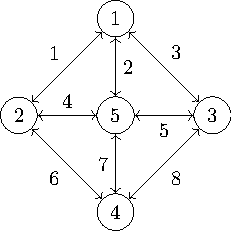
\includegraphics[keepaspectratio,width=1.0\textwidth,height=0.35\textheight]{chapters/tsp/figs/ugraph-figure0}
\caption{\label{fig:tsp:ugraph}Sample weighted graph G with at least one Hamiltonian Cycle}
\end{figure}

Consider a digraph G such as that in \cref{fig:tsp:ugraph}.  Ordinarily this would be shown as an undirected graph because all arcs are two-way, but it is presented as an equivalent directed graph so that it more closely matches the input digraphs as described for the \gls{cps} rules described above, specifically regarding the set \(E\) of arc subcells.  A quick examination will show that there is at least one Hamiltonian Cycle in this digraph, and thus there will be at least one Hamiltonian Cycle with the minimum total weight.  \Cref{fig:tsp:utree} is a tree diagram showing the logical progression of the algorithm as applied to this digraph, assuming that vertex 1 is selected as the root of the Hamiltonian Cycle.  Vertices in bold are the ends of the paths with a minimum cost, while vertices in italics are the ends of the paths where there is no arc in the digraph such that a Hamiltonian Cycle can be completed, based on the digraph traversal up to that point.  The arcs are labelled with the cumulative weight of the path taken to reach the lower vertex.

\begin{figure}
\centering
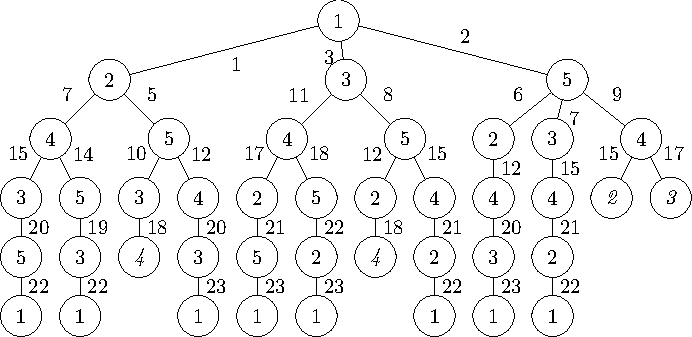
\includegraphics[keepaspectratio,width=1.0\textwidth,height=0.35\textheight]{chapters/tsp/figs/ugraph-figure1}
\caption[A tree diagram representing all potential evolutions of the \gls{cps} \acrlong{tsp} algorithm on the graph in \cref{fig:tsp:ugraph}]{\label{fig:tsp:utree}Tree diagram of the algorithm in action on graph G}
\end{figure}

\begin{cpobjectsfloat}
\begin{cpobjects}
    \cpobjectsline{\cpfunc{e}{\cpfunc{f}{1}\,\cpfunc{t}{2}\,\cpfunc{w}{1}} \; \cpfunc{e}{\cpfunc{f}{1}\,\cpfunc{t}{3}\,\cpfunc{w}{3}} \; \cpfunc{e}{\cpfunc{f}{1}\,\cpfunc{t}{5}\,\cpfunc{w}{2}} \; \cpfunc{e}{\cpfunc{f}{2}\,\cpfunc{t}{1}\,\cpfunc{w}{1}}}%
    \cpobjectsline{\cpfunc{e}{\cpfunc{f}{2}\,\cpfunc{t}{4}\,\cpfunc{w}{6}} \; \cpfunc{e}{\cpfunc{f}{2}\,\cpfunc{t}{5}\,\cpfunc{w}{4}} \; \cpfunc{e}{\cpfunc{f}{3}\,\cpfunc{t}{1}\,\cpfunc{w}{3}} \; \cpfunc{e}{\cpfunc{f}{3}\,\cpfunc{t}{4}\,\cpfunc{w}{8}}}%
    \cpobjectsline{\cpfunc{e}{\cpfunc{f}{3}\,\cpfunc{t}{5}\,\cpfunc{w}{5}} \; \cpfunc{e}{\cpfunc{f}{4}\,\cpfunc{t}{2}\,\cpfunc{w}{6}} \; \cpfunc{e}{\cpfunc{f}{4}\,\cpfunc{t}{3}\,\cpfunc{w}{8}} \; \cpfunc{e}{\cpfunc{f}{4}\,\cpfunc{t}{5}\,\cpfunc{w}{7}}}%
    \cpobjectsline{\cpfunc{e}{\cpfunc{f}{5}\,\cpfunc{t}{1}\,\cpfunc{w}{2}} \; \cpfunc{e}{\cpfunc{f}{5}\,\cpfunc{t}{2}\,\cpfunc{w}{4}} \; \cpfunc{e}{\cpfunc{f}{5}\,\cpfunc{t}{3}\,\cpfunc{w}{5}} \; \cpfunc{e}{\cpfunc{f}{5}\,\cpfunc{t}{4}\,\cpfunc{w}{7}}}%
    \cpobjectsline{\cpfunc{v}{\cpfunc{v}{1} \, \cpfunc{v}{2} \, \cpfunc{v}{3} \, \cpfunc{v}{4} \, \cpfunc{v}{5}}}
\end{cpobjects}
\caption[Starting set of subcells from \cref{fig:tsp:utree}]{\label{objs:tsp:obj1}Set of subcells from G in the skin membrane at the initial state}
\end{cpobjectsfloat}

The set of subcells contained inside the membrane at various points in the system's evolution are shown in \crefrange{objs:tsp:obj1}{objs:tsp:obj4} (for legibility, when specifying the \(p\) subcells, \cref{objs:tsp:obj4} adopts the compact presentation style for lists set out above in \cref{sec:cps:lists}).  The system starts with the subcells shown in \cref{objs:tsp:obj1}, and the algorithm starts by applying rule 1, randomly selecting vertex 1 as the starting point of the Hamiltonian Cycle and creating the origin subcell \(\cpfunc{s}{\dots}\) (full details of the contents of the subcells are provided in the figures), as shown in \cref{objs:tsp:obj2}.

\begin{cpobjectsfloat}
\begin{cpobjects}
    \cpobjectsline{\cpfunc{e}{\cpfunc{f}{1}\,\cpfunc{t}{2}\,\cpfunc{w}{1}} \quad \cdots \quad \cpfunc{e}{\cpfunc{f}{5} \, \cpfunc{t}{4} \, \cpfunc{w}{7}}}
    \cpobjectsline{\cpfunc{s}{\cpfunc{r}{1} \; \cpfunc{u}{\cpfunc{v}{2} \, \cpfunc{v}{3} \, \cpfunc{v}{4} \cpfunc{v}{5}} \; \cpfunc{p}{\cpfunc{h}{1} \cpfunc{p}{\cpempty}} \; \cpfunc{c}{0}}}
\end{cpobjects}
\caption{\label{objs:tsp:obj2}Set of subcells in the skin membrane after the application of rule one}
\end{cpobjectsfloat}

Next, rule 3 is applied, creating the first level of subcells in the exploration tree.  This creates new \(\cpfunc{s}{\cpfunc{r}{R} \, \cpfunc{u}{\dots} \, \cpfunc{p}{\cpfunc{h}{\dots} \cpfunc{p}{\cpfunc{h}{1} \cpfunc{p}{\cpempty}}} \, \cpfunc{c}{\dots}}\) subcells, representing the potential paths of the cycle after one step.  Rule 4 concurrently removes the old \(s\) subcells from the system.  \Cref{objs:tsp:obj3} shows the subcells within the top-level cell at the end of this first application of rules 3 and 4.

\begin{cpobjectsfloat}
\begin{cpobjects}
    \cpobjectsline{\cpfunc{e}{\cpfunc{f}{1}\,\cpfunc{t}{2}\,\cpfunc{w}{1}} \quad \cdots \quad \cpfunc{e}{\cpfunc{f}{5} \, \cpfunc{t}{4} \, \cpfunc{w}{7}}}
    \cpobjectsline{\cpfunc{s}{\cpfunc{r}{1} \; \cpfunc{u}{\cpfunc{v}{3} \, \cpfunc{v}{4} \cpfunc{v}{5}} \; \cpfunc{p}{\cpfunc{h}{2} \cpfunc{p}{\cpfunc{h}{1} \cpfunc{p}{\cpempty}}} \; \cpfunc{c}{1}}}
    \cpobjectsline{\cpfunc{s}{\cpfunc{r}{1} \; \cpfunc{u}{\cpfunc{v}{2} \, \cpfunc{v}{4} \cpfunc{v}{5}} \; \cpfunc{p}{\cpfunc{h}{3} \cpfunc{p}{\cpfunc{h}{1} \cpfunc{p}{\cpempty}}} \; \cpfunc{c}{3}}}
    \cpobjectsline{\cpfunc{s}{\cpfunc{r}{1} \; \cpfunc{u}{\cpfunc{v}{2} \, \cpfunc{v}{3} \cpfunc{v}{4}} \; \cpfunc{p}{\cpfunc{h}{2} \cpfunc{p}{\cpfunc{h}{5} \cpfunc{p}{\cpempty}}} \; \cpfunc{c}{2}}}
\end{cpobjects}
\caption{\label{objs:tsp:obj3}Set of subcells in the skin membrane after a single application of rules three and four}
\end{cpobjectsfloat}

Eventually, after repeating rules 3 and 4 five times, rule 2 becomes applicable.  At this point, rule 2 is applied, creating the \(z\) subcells that represent the final arc traversal from another vertex back to the origin vertex, vertex 1.  Finally, rule 5 selects one of those \(z\) subcells with minimum cost as the solution, and outputs the path and cost subcells relating to that cycle.  \Cref{objs:tsp:obj4} outlines the subcells present in the system at this end point.

\begin{cpobjectsfloat}
\begin{cpobjects}
    \cpobjectsline{\cpfunc{e}{\cpfunc{f}{1}\,\cpfunc{t}{2}\,\cpfunc{w}{1}} \quad \cdots \quad \cpfunc{e}{\cpfunc{f}{5} \, \cpfunc{t}{4} \, \cpfunc{w}{7}}}
    \cpobjectsline{\cpfunc{z}{\cpfunc{c}{22} \; \cpfunc{p}{1|5|3|4|2|1}} \quad \cdots \quad \cpfunc{z}{\cpfunc{c}{22} \; \cpfunc{p}{1|2|4|3|5|1}}}
    \cpobjectsline{\cpfunc{c'}{22} \quad \cpfunc{p'}{1|5|3|4|2|1}}
\end{cpobjects}
\caption[Set of subcells in the skin membrane at completion of the computation]{\label{objs:tsp:obj4}Set of subcells in the skin membrane at completion of the computation, if rule 5 selects the subcell containing the path subcell representing the traversals 1 - 2 - 4 - 3 - 5 - 1.}
\end{cpobjectsfloat}

To illustrate the progression of the algorithm through various branches of the exploration tree, consider the following examples, each beginning with the \(\cpfunc{s}{\dots}\) and set of \(\cpfunc{e}{\dots}\) subcells illustrated in \cref{objs:tsp:obj2}.

From \(\cpfunc{s}{\cpfunc{r}{1} ~ \,\cpfunc{u}{\cpfunc{v}{2}\,\cpfunc{v}{3}\,\cpfunc{v}{4}\,\cpfunc{v}{5}}\, ~ \cpfunc{p}{\cpfunc{h}{1}\cpfunc{p}{\cpempty}} ~ \,\cpfunc{c}{0}}\), the subcell representing the beginning of the cycle at vertex 1, rule 3 will create, among others, an \(\cpfunc{s}{\cpfunc{r}{1} ~ \,\cpfunc{u}{\cpfunc{v}{3}\,\cpfunc{v}{4}\,\cpfunc{v}{5}} ~ \,\cpfunc{p}{\cpfunc{h}{2}\cpfunc{p}{\cpfunc{h}{1}\cpfunc{p}{\cpempty}}} ~ \,\cpfunc{c}{1}}\) subcell representing an arc traversal to vertex 2 with a weight subcell \(\cpfunc{c}{1}\).  In turn, another new subcell, among others, will be derived from this subcell representing a further arc traversal to vertex 4, with a weight subcell of \(\cpfunc{c}{7}\).  This continues for subcells representing traversals to vertices 3 (\(\cpfunc{c}{15}\)) and 5 (\(\cpfunc{c}{20}\)), until finally the latter subcell contains an empty \(u\) subcell.  For this subcell, rule 2 finds an \(e\) subcell that connects vertex 5 to \(R\), the root vertex 1, and so creates a \(z\) subcell (the top \(z\) subcell in \cref{objs:tsp:obj4}) containing a \(\cpfunc{p}{\dots}\) subcell representing the traversed path, and a subcell \(\cpfunc{c}{22}\), representing the total cost of the cycle.  This final subcell is potentially selected at random by rule 5, because 22 is the minimum cost possible in this particular digraph, when starting and finishing at vertex 1.

Conversely, another chain of subcell creations will occur as vertex 1 to vertex 5, with \(\cpfunc{c}{2}\), vertex 5 to vertex 4 with \(\cpfunc{c}{9}\), vertex 4 to vertex 2 with weight \(\cpfunc{c}{15}\).  At this point, \(\cpfunc{u}{\cpfunc{v}{3}}\) is non-empty, but there is no \(e\) subcell representing a transition from vertex 2 to vertex 3, so this subcell reaches a `dead-end', and will be removed without further effect by rule 4.

Similarly, a progression will occur from vertex 1 to vertex 3 with \(\cpfunc{c}{3}\), to vertex 5 with \(\cpfunc{c}{8}\), to vertex 2 with \(\cpfunc{c}{12}\), and to vertex 4 with \(\cpfunc{c}{18}\).  At this point, every vertex has been visited, and the subcell \(u\) in this particular \(s\) subcell is empty, but there is no \(e\) subcell representing a transition from the current vertex back to the origin, so no \(z\) subcell will be created based on it.

%-------------------------------------------

\subsection{Directed Graph Example}
While the above example is drawn as a directed graph, to better match with the specification of the edges in the set of subcells \(E\), it was effectively an undirected graph.  To demonstrate that the \gls{tsp} algorithm is at least as effective in the directed case, \cref{fig:tsp:ugraph} was modified to remove some bidirectional arcs.  The modified digraph is presented in \cref{fig:tsp:digraph} and the accompanying exploration tree in \cref{fig:tsp:dtree}.  The updated set of subcells that are inside the skin membrane at the start of the computation are shown in \cref{objs:tsp:obj1d}.  The changes made are that the edges from 1 to 2 and from 5 to 3 have been removed, and the weights between 1 and 3 and 4 and 5 have been partially modified so that they are different in each direction.

\begin{figure}
\centering
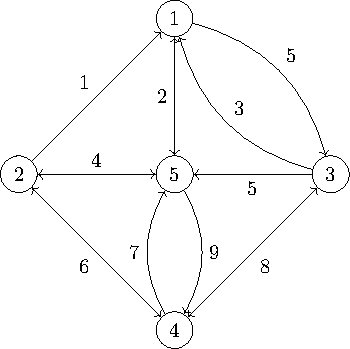
\includegraphics[keepaspectratio,width=1.0\textwidth,height=0.35\textheight]{chapters/tsp/figs/ugraph-figure2}
\caption{\label{fig:tsp:digraph}Sample weighted digraph H with at least one Hamiltonian Cycle}
\end{figure}

\begin{figure}
\centering
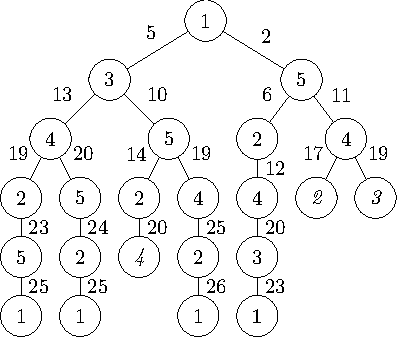
\includegraphics[keepaspectratio,width=1.0\textwidth,height=0.35\textheight]{chapters/tsp/figs/ugraph-figure3}
\caption[Tree diagram of the algorithm's operation on a directed graph]{\label{fig:tsp:dtree}Tree diagram of the algorithm in action on the second, directed graph, H}
\end{figure}

\begin{cpobjectsfloat}
\begin{cpobjects}
    \cpobjectsline{\mathbf{\cpfunc{e}{\mathbf{\cpfunc{f}{1}\,\cpfunc{t}{3}\,\cpfunc{w}{5}}}} \quad \cpfunc{e}{\cpfunc{f}{1}\,\cpfunc{t}{5}\,\cpfunc{w}{2}} \quad \cpfunc{e}{\cpfunc{f}{2}\,\cpfunc{t}{1}\,\cpfunc{w}{1}}}%
    \cpobjectsline{\cpfunc{e}{\cpfunc{f}{2}\,\cpfunc{t}{4}\,\cpfunc{w}{6}} \quad \cpfunc{e}{\cpfunc{f}{2}\,\cpfunc{t}{5}\,\cpfunc{w}{4}} \quad \cpfunc{e}{\cpfunc{f}{3}\,\cpfunc{t}{1}\,\cpfunc{w}{3}} \quad \cpfunc{e}{\cpfunc{f}{3}\,\cpfunc{t}{4}\,\cpfunc{w}{8}}}%
    \cpobjectsline{\cpfunc{e}{\cpfunc{f}{3}\,\cpfunc{t}{5}\,\cpfunc{w}{5}} \quad \cpfunc{e}{\cpfunc{f}{4}\,\cpfunc{t}{2}\,\cpfunc{w}{6}} \quad \cpfunc{e}{\cpfunc{f}{4}\,\cpfunc{t}{3}\,\cpfunc{w}{8}} \quad \cpfunc{e}{\cpfunc{f}{4}\,\cpfunc{t}{5}\,\cpfunc{w}{7}}}%
    \cpobjectsline{\cpfunc{e}{\cpfunc{f}{5}\,\cpfunc{t}{1}\,\cpfunc{w}{2}} \quad \cpfunc{e}{\cpfunc{f}{5}\,\cpfunc{t}{2}\,\cpfunc{w}{4}} \quad \mathbf{\cpfunc{e}{\mathbf{\cpfunc{f}{5}\,\cpfunc{t}{4}\,\cpfunc{w}{9}}}}}%
    \cpobjectsline{\cpfunc{v}{\cpfunc{v}{1} \, \cpfunc{v}{2} \, \cpfunc{v}{3} \, \cpfunc{v}{4} \, \cpfunc{v}{5}}}
\end{cpobjects}
    \caption[Set of subcells from H in the skin membrane at the initial state]{\label{objs:tsp:obj1d}Set of subcells from H in the skin membrane at the initial state (those different from G are in bold)}
\end{cpobjectsfloat}

These modifications have a significant effect upon the evolution of the system.  There are fewer potential paths through the digraph, which results in the instantiation of fewer subcells, and so the exploration tree is consequently narrower.  Thus, this particular application of the algorithm has a lower maximum space complexity.  Note though that there is absolutely no change in the operation of the algorithm.  The differences in the \(e\) subcells present at the start of the evolution of the system lead to a different result, without any change in the application of the rules.

%----------------------------------------